\documentclass[11pt]{ieeeconf}
\usepackage{graphicx}
\usepackage{float}
\usepackage{lettrine}
\usepackage{caption}
\usepackage{url}


\newcommand\blfootnote[1]{%
  \begingroup
  \renewcommand\thefootnote{}\footnote{#1}%
  \addtocounter{footnote}{-1}%
  \endgroup
}

\title{Bumper Car Sumo}
\author{Jaden Simon - simonjaden223@gmail.com \\ \and
	   Melvin Bosnjak - meco0597@gmail.com \\ \and
	   Daniel Humeniuk - d.humeniuk@utah.edu \\ \and
	   http://bumpercarsumo.weebly.com/}

%Herein is our final report

%Professor Stevens' requirements for the report bellow

%Make sure you take time for your technical documentation! The final technical report can be completed the week following your project demonstration. Don't forget to plan for that! The final technical document will be written in LaTeX and will require formatting as the two column IEEE conference or journal paper as was done in 3991.

%This aspect of the project is critical to ensure that you are communicating well with the instructor as to the status of your project. This portion of the grade will be based on the weekly logs and team meetings that you have with the instructor. It is critical that you understand the progress of your project and that you are able to communicate that to your team members and the instructor. This serves as an early warning system in such instances as when risks can not be reduced or worst case scenarios play out, when the required engineering effort was under estimated, or when parts don't arrive or a team member is not delivering or needs help to keep from becoming a roadblock to progress of the project. It takes discipline to manage a team, and this grade is part of that. You will be recorded 0.67% of your grade for each week's team log. If you don't turn one in, you will not get any points for that week. If the log is insufficient, you will get half credit for that week. A log is insufficient if it is not clear what progress has been made during the week, whether the project is on schedule, and what the current perceived risks are that could prevent delivering on the project specifications by demo day.

%Part of the reporting is meeting with the instructor. These meetings can be as often as every week, depending on the need of the team. Some of these meetings will be mini design reviews, others will be status and risk updates. Use the instructor and outside resources to help your project be a smashing success! Make sure you acknowledge the help of others in your technical report. 
	   
\begin{document}

\maketitle

\begin{abstract}
BumperCarSumo is a fully interactive multiplayer game. Each player controls a little robot on a designated play area. A robot is controlled by a central game hub that communicates to the robots via WiFi. The controllers are connected to the hub with the use of Bluetooth technology. The robots are powered internally with a rechargable lithium ion battery and moves about the play area with geared DC Motors. The goal of the game is to be the last remaining player on the play area by any means possible. Once a player has fallen off of the play area, the player has lost the match. The hub tracks each robot with a web camera and an OpenCV program to ensure that once it has fallen off the play area, the robot will turn off and remains off until the next game. Once all but one player remains, the round is over and is free to be played again.
\end{abstract}
%This is all taken from 2018 requirements of the report and will be updated as needed

\section{Introduction}
%Introduction and motivation (describe the problem, and who cares if you solve it)
The purpose of BumperCarSumo is to provide entertainment that mirrors popular Battle Royale game play with the use of physically controlled objects. The components currently required for game play is a white play area, a dark (black if possible) out of bounds zone, a web camera, a Raspberry Pi 3 B+, the BumperCarSumo program loaded onto the Raspberry Pi, two to four remote controlled robots, and the corresponding amount of controllers. Each component will be described throughout this report. 

\section{Background}

%Background (What other things are out there that you're drawing from? Are there similar things that you're referencing or extending?)

The concept of BumperCarSumo originated from a desire to control robots and stage a free-for-all match between players. Battle Royale video games have become a huge success in recent years and we wanted to attempt similar style of ''last man standing'' with these remote controlled robots.

The concept of the robots came from the Ollie Sphero. The comparison of the Ollie and our design can be seen in Figure \ref{Ollie}. Our design came out much bigger than expected due to the gears required to slow the motor down. The motors also created another reason for more space. The material used for traction was much simpler as we were intending for the robots to be able to slide if hit but still able to maintain a grip on the play area.

\begin{figure}[H]
\centering
\captionsetup{justification=centering}
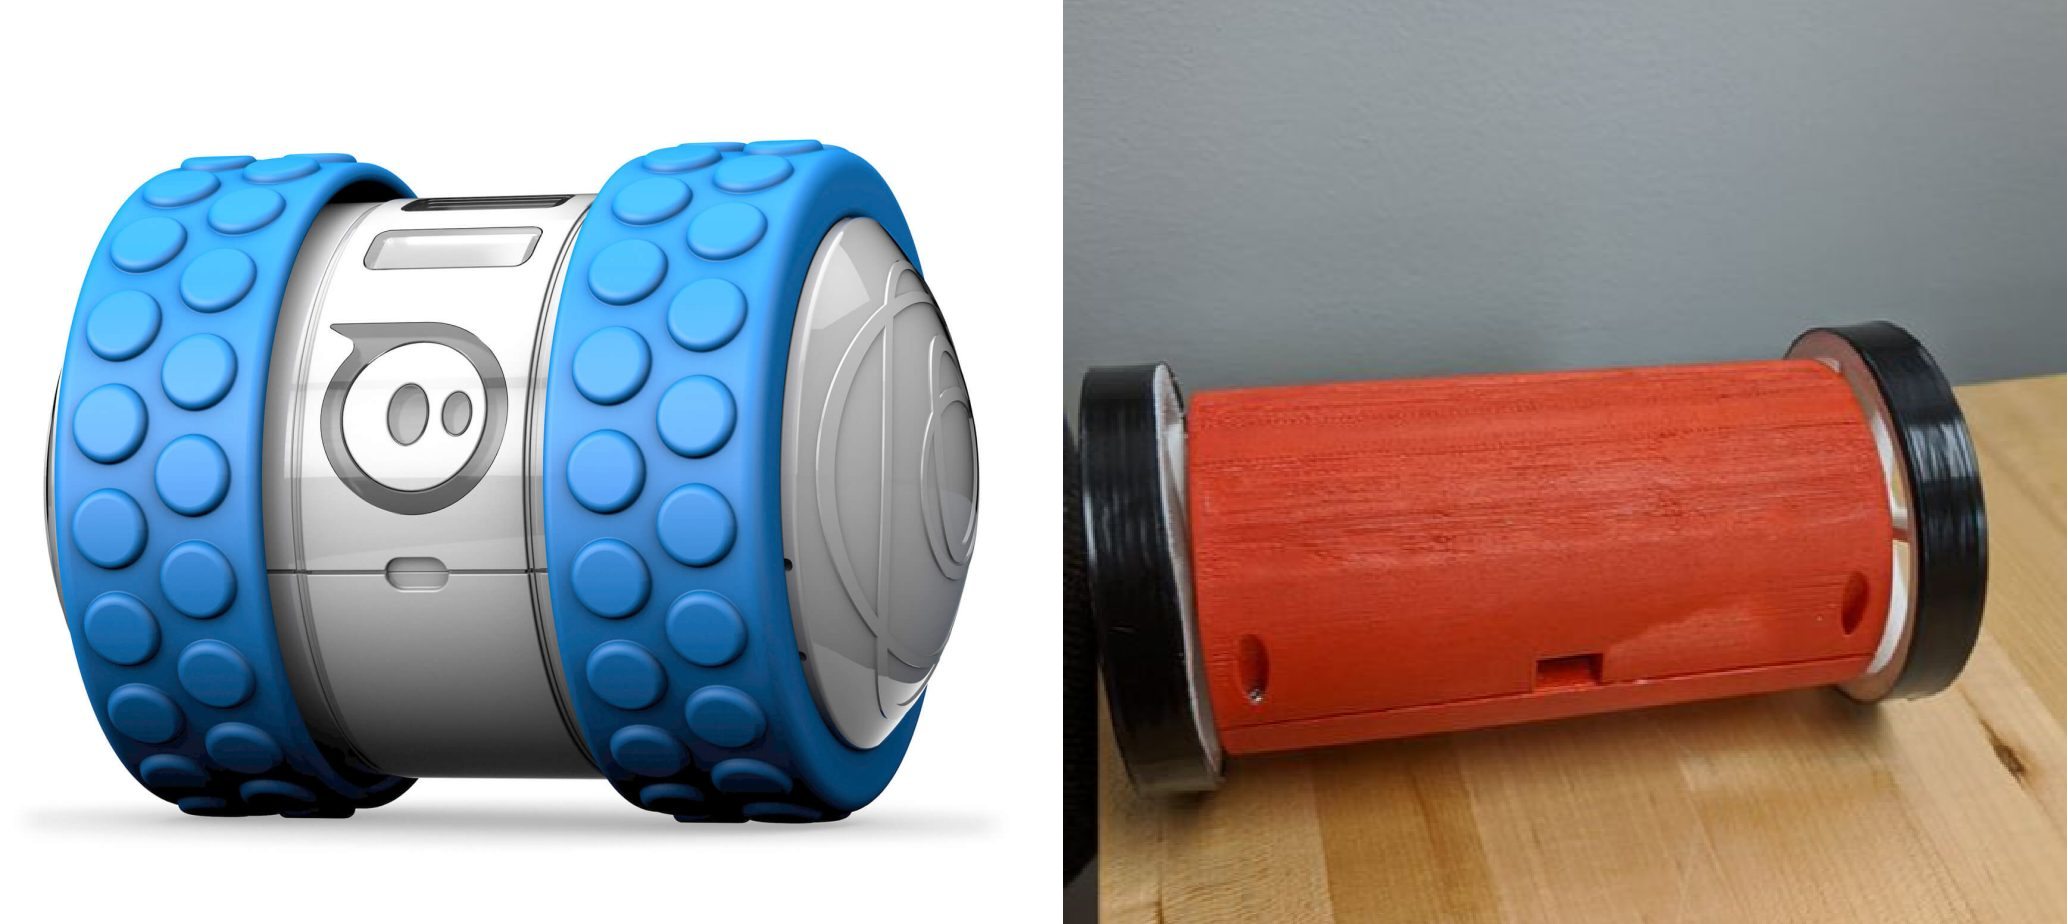
\includegraphics[width=0.5\textwidth]{images/SideBySide.png}
\caption{The Ollie from Sphero comparied with our Design\\Source: Adapted from \cite{ollie:19}}
\label{Ollie}
\end{figure}


\section{Project Implementation}
%Project Implementation (The details of what you did, what you used, and why you made the choices you did. This is likely to be by far the largest section of your report, and can have multiple sub-sections) 

The central piece of the game is the Game Hub. This Hub is constructed with a Raspberry Pi 3 B+ which included enough features to make the gameplay possible. The robots are PCBs and DC Motors wrapped in a 3D printed shell. Each PCB receives commands from the Game Hub via WiFi. Players control each robot with the use of a Wii Balance Board which is connected to the Hub through Bluetooth. The web camera is connected to the Game Hub with USB and detects the unique color of each robot. The play area is a 4ft round surface in which the robots are able to move around and play. The camera sits above the play area on an 8ft post. Each component of the project is described in more detail below. 

\subsection{The Game Hub}

We utilized a Raspberry Pi 3 B+ as our game hub. The device contained both Bluetooth and WiFi capabilities which was critical for communicating to the external game peripherals. The Pi was an excellent choice as it is small, portable, and capable enough to handle the software required for the game. 

The controllers were connected to the Game Hub via Bluetooth. The controllers are based on Wii Balance Boards. The Game Hub starts the controller logic in a separate thread and once connected, continuously polls the Bluetooth devices to ensure they stay connected. When a game is in progress, the data collected from Bluetooth is processed. Once processed, the Game Hub will determine in which direction the player is leaning and send the corresponding command to the player's robot.

\subsection{Controllers}
For our controllers, we used the Wii Balance Board. Our intention behind this controller system was to add layers of complexity and extra challenges to gameplay. The interface was an opensource library found on github. There were a few versions of the library but we electected to use the library written in Python. We made an API for our purposes to be as simple as possible with only two functions that connected to a board and collected the data from the board.

Our API relied on a single WiiController object that connected to multiple boards. The functions of the API are start and get\_data. The start function accepts the MAC Address of one of our boards and instantiated the board to a corresponding WiiBoard object board1, board2, board3, or board4. Once connected, the board will need to be continously polled to ensure the Bluetooth stayed connected. The get\_data function accepts the MAC Address of one Balance board and an array of that board's data would be returned to the Hub. The Hub then processes this data and sends the proper commands to the corresponding robot.

\subsection{Robots}

The robots are a mix of hardware and software. A PCB lies within each robot that contains an ESP-12F. The ESP-12F runs custom software that drives the robot. We printed custom shells and wheels to protect and drive the robots. The custom hardware and software made debugging the robots a challenge but a worthwhile effort nonetheless. 

\begin{figure}[H]
\centering
\captionsetup{justification=centering}
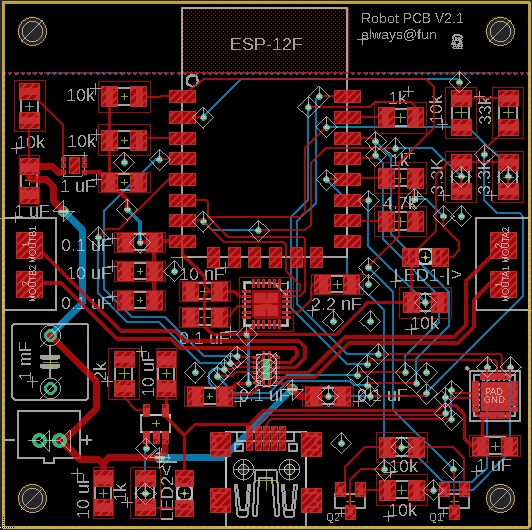
\includegraphics[width=0.5\textwidth]{images/FinalPCB.jpg}
\caption{The custom PCB that controls each robot}
\label{PCB}
\end{figure}

The custom hardware lies in the PCB which can be seen in Figure \ref{PCB}. The PCB contains 4 mounting pads, 2 for each DC Motor that drives the robot, as well as M2.5 drill holes on each corner. The drill holes allowed for the PCBs to be mounted within the shell as seen in Figure \ref{shell}. The ESP-12F chip on the PCB was programmed with the use of USB and a CP2104 programmer chip on the board. An MPU is located in the center of the PCB. The MPU was integrated as a backup to the camera detection. The data from the MPU would allow us to determine if the robot had fallen from the board. This was later discarded as our Computer Vision portion of the project worked as expected. A DRV Motor Driver is included on the PCB to allow for the DC Motors to spin both forward and backward. A LDO chip was also added to handle voltage dropouts. 

The software in the ESP-12F is responsible for receiving data from the Game Hub via WiFi and converting that data to voltages delivered to the DC Motors.  

\begin{figure}[H]
\centering
\captionsetup{justification=centering}
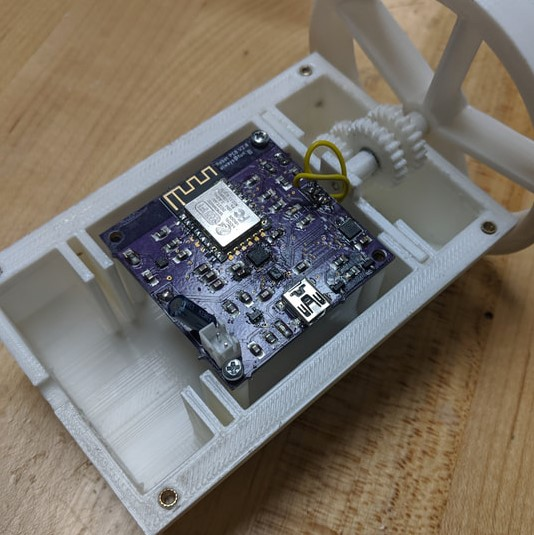
\includegraphics[width=0.5\textwidth]{images/Shell.png}
\caption{A snapshot of the insides of the robot shell}
\label{shell}
\end{figure}

\subsection{The Camera}



\subsection{The Play Area}

The play area is simple in nature but plays an essential part in the overall game. We painted the table top white and covered the floor black with a sheet. As described in the camera section, every color that would enter the black region would be filtered out. The most complex piece of the play area was the 8ft pole which held the camera. It was essential the camera be at this height as to ensure all players in the area would be caputed. We were lucky enough to get a table that sat enough off the ground that would not allow a player to reenter the game if a glitch with the Computer Vision were to occur. This would cause other problems but during the demo day, this proved to be a nonissue. 

\section{Discoveries}
%Discoveries and pitfalls (things you learned and things that other groups would find helpful)

We learned pretty quick that the original DC motors we were using were far too powerful for such a small play area. The motors offered over 1000 RPM which can be handled with gearing the motors. The unfortunate result of this, however, was the small area in which the gears were to fit. The first few attempts at gearing the motors were a success in many ways and a failure in others. The gears did work and we were able to get a simple gear test box working as seen in Figure \ref{gears}. The gears faced problems with proper meshing, resulting in small pieces of PLA to fly from the test box. With lubrication, the problem continued still. 

\begin{figure}[H]
\centering
\captionsetup{justification=centering}
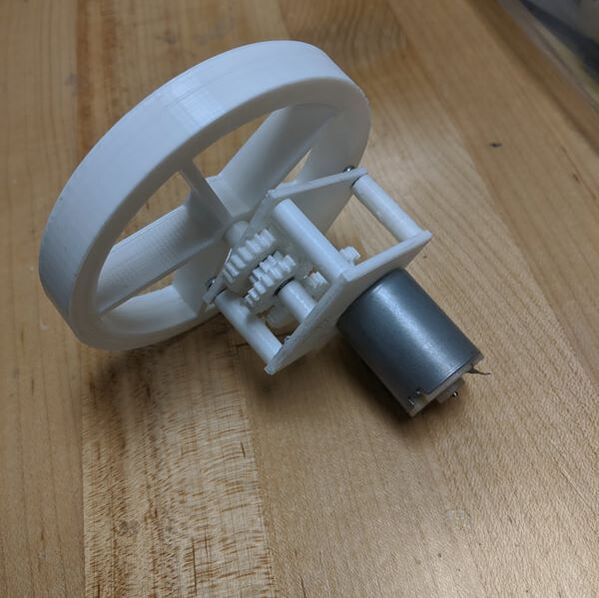
\includegraphics[width=0.5\textwidth]{images/GearTest.jpg}
\caption{The first ideration of the designed gears}
\label{gears}
\end{figure}

GEARS SUCK!

\section{Evaluation}
%How well did it work - be honest here - if there were things that didn't work out the way you expected, write about them too. Also make sure to describe your testing and evaluation strategy. Don't just say it worked - describe how you know it worked, and even what "worked" means. This is likely to be the second-largest section in your report.

GEARS MADE IT SUCK!

\section{Bill of Materials}
% Bill of materials (or at least a list of all the materials, equipment, etc. that you used. You don't need prices here, but you should include a list of things you used)

Our project cost a whopping 900 dollary doos!

\section{Conclusion}
%- Conclusions (wrap things up with some final text. Include a pointer to your final web site.) 

\bibliographystyle{IEEEtran}
\bibliography{IEEEabrv,bib/ref}

\end{document}